% Copyright 2020  Ed Bueler

\documentclass[10pt,hyperref]{beamer}

\mode<presentation>{
  \usetheme{Madrid}
  \usecolortheme{beaver}
  \setbeamercovered{transparent}  
  \setbeamerfont{frametitle}{size=\large}
}

\setbeamercolor*{block title}{bg=red!10}
\setbeamercolor*{block body}{bg=red!5}

\usepackage[english]{babel}
\usepackage[latin1]{inputenc}
\usepackage{times}
\usepackage[T1]{fontenc}
% Or whatever. Note that the encoding and the font should match. If T1
% does not look nice, try deleting the line with the fontenc.

\usepackage{empheq}
\usepackage{xspace}
\usepackage{verbatim,fancyvrb}

\usepackage{tikz}
\usetikzlibrary{shapes,arrows.meta,decorations.markings,decorations.pathreplacing,fadings,positioning}

\usepackage{hyperref}

% If you wish to uncover everything in a step-wise fashion, uncomment
% the following command: 
%\beamerdefaultoverlayspecification{<+->}

\newcommand{\ba}{\mathbf{a}}
\newcommand{\bb}{\mathbf{b}}
\newcommand{\bc}{\mathbf{c}}
\newcommand{\bg}{\mathbf{g}}
\newcommand{\bq}{\mathbf{q}}
\newcommand{\br}{\mathbf{r}}
\newcommand{\bx}{\mathbf{x}}
\newcommand{\by}{\mathbf{y}}
\newcommand{\bv}{\mathbf{v}}
\newcommand{\bu}{\mathbf{u}}
\newcommand{\bw}{\mathbf{w}}

\newcommand{\bF}{\mathbf{F}}

\newcommand{\grad}{\nabla}
\newcommand{\Div}{\nabla\cdot}

\newcommand{\CC}{\mathbb{C}}
\newcommand{\RR}{\mathbb{R}}

\newcommand{\ddt}[1]{\ensuremath{\frac{\partial #1}{\partial t}}}
\newcommand{\ddx}[1]{\ensuremath{\frac{\partial #1}{\partial x}}}
\newcommand{\Matlab}{\textsc{Matlab}\xspace}
\newcommand{\Octave}{\textsc{Octave}\xspace}
\newcommand{\MO}{\Matlab}
\newcommand{\eps}{\epsilon}

\newcommand{\ip}[2]{\left<#1,#2\right>}

\newcommand{\trefcolumn}[1]{\begin{bmatrix} \phantom{x} \\ #1 \\ \phantom{x} \end{bmatrix}}
\newcommand{\trefmatrixtwo}[2]{\left[\begin{array}{c|c|c} & & \\ #1 & \dots & #2 \\ & & \end{array}\right]}
\newcommand{\trefmatrixthree}[3]{\left[\begin{array}{c|c|c|c} & & & \\ #1 & #2 & \dots & #3 \\ & & & \end{array}\right]}
\newcommand{\trefmatrixgroups}[4]{\left[\begin{array}{c|c|c|c|c|c} & & & & & \\ #1 & \dots & #2 & #3 & \dots & #4 \\ & & & & & \end{array}\right]}

\newcommand{\blocktwo}[4]{\left[\begin{array}{c|c} #1 & #2 \\ \hline #3 & #4 \end{array}\right]}

\newcommand{\bqed}{{\color{blue}\qed}}

\newcommand{\exer}[2]{\medskip\noindent \textbf{#1.}\quad #2}


\AtBeginSection[]
{
  \begin{frame}<beamer>
    \frametitle{Outline}
    \tableofcontents[currentsection,hideallsubsections]
  \end{frame}
}

\title[Finite volume methods]{Finite volume methods for \\ advection equations and hyperbolic systems}

%\subtitle{part I: xx}

\author{Ed Bueler}

\institute[UAF]{University of Alaska Fairbanks}

\date{June 2020}


\begin{document}
\beamertemplatenavigationsymbolsempty

\begin{frame}
  \maketitle
\end{frame}


\section{scalar advection equation}

\begin{frame}[fragile]
\frametitle{overview}

\begin{itemize}
\item slides about numerical solutions of first-order PDEs
    \begin{itemize}
    \item[$\circ$] genuinely introductory!
    \end{itemize}
\item we will solve this tree of equations:

\newcommand\mynum[1]{{\renewcommand{\insertenumlabel}{#1}%
      \usebeamertemplate{enumerate item} \,}}

\bigskip
\begin{center}
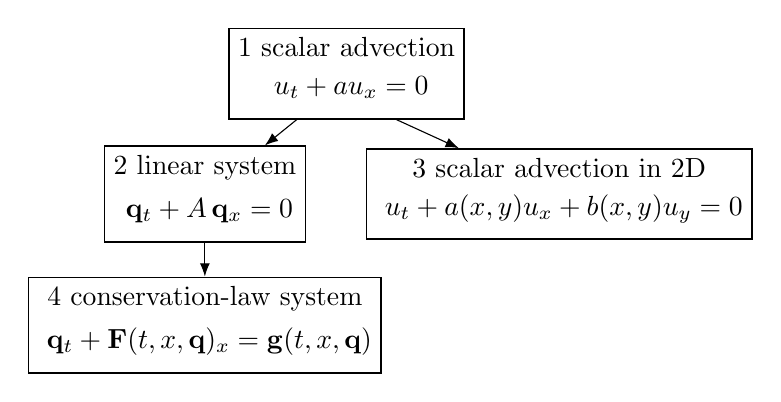
\begin{tikzpicture}[scale=0.9,
                    >={Latex[length=2mm]},
  eqn/.style={
     rectangle,draw,fill=white,align=center,line width=0.6pt,minimum width=15mm}]

%center
\draw[line width=1pt] (0,0)     node[eqn] (scalaradvect)  {\mynum{1} scalar advection \\ {\Large \strut} $u_t + a u_x=0$};
\draw[line width=1pt] (3,-1.7)     node[eqn] (scalartwod)  {\mynum{3} scalar advection in 2D \\ {\Large \strut} $u_t + a(x,y) u_x + b(x,y) u_y=0$};
\draw[line width=1pt] (-2,-1.7)    node[eqn] (linearsystem)  {\mynum{2} linear system \\ {\Large \strut} $\bq_t + A\, \bq_x=0$};
\draw[line width=1pt] (-2,-3.55)    node[eqn] (generalsystem)  {\mynum{4} conservation-law system \\ {\Large \strut} $\bq_t + \bF(t,x,\bq)_x=\bg(t,x,\bq)$};

\path[-Latex]
   ([xshift=-2em]scalaradvect.south) edge node {} (linearsystem)
   ([xshift=2em]scalaradvect.south) edge node {} (scalartwod)
   (linearsystem.south) edge node {} (generalsystem);
\end{tikzpicture}

\bigskip
    \begin{itemize}
    \item[$\circ$] arrows show generalizations
    \end{itemize}
\end{center}

\end{itemize}
\end{frame}


\begin{frame}{solution by characteristics}

\begin{itemize}
\item the \emph{scalar advection equation}:
    $$u_t + a u_x=0$$
    \begin{itemize}
    \item[$\circ$] we will only need $a\in\RR$ constant, so let's assume that
    \end{itemize}
\item x
\end{itemize}
\end{frame}


\begin{frame}{upwind and Lax-Wendroff schemes}

\begin{itemize}
\item x
\end{itemize}
\end{frame}


\begin{frame}{results}

\begin{itemize}
\item results from short \Matlab code\footnote{\href{http://bueler.github.io/codes/adcompare.m}{\texttt{bueler.github.io/codes/adcompare.m}}}
\end{itemize}
\end{frame}


\begin{frame}{method-of-lines thinking (MOL)}

\begin{itemize}
\item x
\end{itemize}
\end{frame}


\begin{frame}{Godunov's barrier theorem}

\begin{itemize}
\item x
\end{itemize}

\begin{theorem}[\emph{Godunov's barrier theorem, 1959}]  A monotonicity-preserving linear scheme for the 1D constant-coefficient equation $u_t + \alpha u_x=0$ cannot have second-order (or higher) local truncation error in $x$.\end{theorem}
\end{frame}


\begin{frame}{x}

\begin{itemize}
\item x
\end{itemize}
\end{frame}


\begin{frame}{x}

\begin{itemize}
\item x
\end{itemize}
\end{frame}


\section{linear systems}

\begin{frame}{x}

\begin{itemize}
\item x
\end{itemize}
\end{frame}


\begin{frame}{x}

\begin{itemize}
\item x
\end{itemize}
\end{frame}



\section{scalar advection in 2D}

\begin{frame}{x}

\begin{itemize}
\item using C using PETSc \dots not shown \dots see \,\href{https://github.com/bueler/p4pdes}{\texttt{github.com/bueler/p4pdes}}
\item x
\end{itemize}
\end{frame}


\section{nonlinear conservation-law systems}

\begin{frame}{x}

\begin{itemize}
\item x
\end{itemize}
\end{frame}


\begin{frame}{x}

\begin{itemize}
\item x
\end{itemize}
\end{frame}


\begin{frame}[fragile]
\frametitle{xx}

\begin{itemize}
\item xx:

\medskip
\begin{Verbatim}[fontsize=\scriptsize]
>> size(A)
ans =
      201        5
\end{Verbatim}

%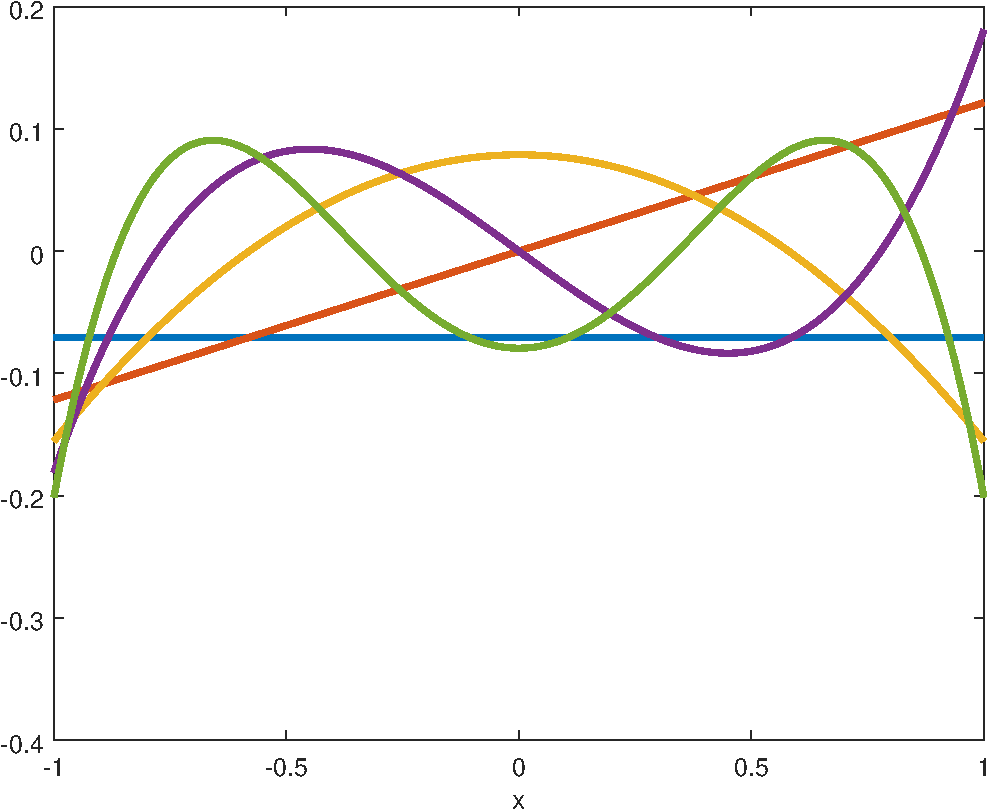
\includegraphics[width=0.55\textwidth]{figs/legendre} \quad 
\end{itemize}
\end{frame}


\end{document}

